% ============================================================================
%  CHAPTER 23 — COMPLETE API REFERENCE
% ============================================================================
\chapter{Complete API Reference}
\label{ch:api-reference}

\epigraph{Good documentation is not about writing less.  It is about
writing enough that the next developer can change the code with
confidence.}{}

This chapter provides exhaustive documentation for every public class,
function, dataclass, and constant exported by the three Python packages
that comprise the PQC Secure MAVLink Tunnel:

\begin{description}
  \item[\texttt{core}] The protocol engine---handshake, AEAD framing,
    proxy, suites, metrics schema, and configuration.
  \item[\texttt{sscheduler}] The drone-side benchmark scheduler---suite
    iteration, remote GCS control, metrics collection, and JSONL output.
  \item[\texttt{scheduler}] The simplified GCS-side scheduler---remote
    command server and proxy lifecycle management.
\end{description}

% ────────────────────────────────────────────────────────────────────────────
\section{\texttt{core} Package Overview}
\label{sec:api-core-overview}

The \texttt{core} package contains 22~Python modules totalling
approximately 10{,}500~lines of code.  Table~\ref{tab:api-core-modules}
summarises every module and its role.

\begin{longtable}{l r p{6.5cm}}
  \caption{Modules in the \texttt{core} package.}
  \label{tab:api-core-modules} \\
  \toprule
  \textbf{Module} & \textbf{Lines} & \textbf{Responsibility} \\
  \midrule
  \endfirsthead
  \toprule
  \textbf{Module} & \textbf{Lines} & \textbf{Responsibility} \\
  \midrule
  \endhead
  \bottomrule
  \endfoot

  \texttt{\_\_init\_\_.py}     & 25    & Package docstring; re-exports nothing. \\
  \texttt{errors.py}           & 40    & Exception hierarchy (6~classes). \\
  \texttt{aead.py}             & 470   & AEAD framing, header serialization, replay window. \\
  \texttt{proxy.py}            & 1{,}665 & Proxy event loop, handshake orchestration, rekey. \\
  \texttt{rate\_limiter.py}    & 139   & Token-bucket rate limiter for handshake admission. \\
  \texttt{config.py}           & 623   & Centralised \texttt{CONFIG} dictionary, env overrides. \\
  \texttt{handshake.py}        & 359   & Wire-format serialization/deserialisation. \\
  \texttt{keygen.py}           & 88    & OQS key generation wrapper. \\
  \texttt{crypto\_utils.py}    & 658   & AEAD primitives, key derivation, OQS wrappers. \\
  \texttt{observability.py}    & 84    & Structured logging, metrics singletons. \\
  \texttt{suites.py}           & 850   & Suite generation, lookup, validation, iteration. \\
  \texttt{keys.py}             & 300   & Key-pair management, file I/O, metadata. \\
  \texttt{metrics\_schema.py}  & 625   & 18~dataclass categories (A--R) + aggregator. \\
  \texttt{collectors.py}       & 766   & Metric collectors (system, process, MAVLink). \\
  \texttt{runner.py}           & 1{,}368 & Proxy lifecycle, subprocess management, auto-mode. \\
  \texttt{scheduler.py}        & 879   & Suite rotation policy engine. \\
  \texttt{time\_utils.py}      & 203   & Monotonic clock, UTC timestamps, duration formatting. \\
  \texttt{process\_mgr.py}     & 998   & Process manager, health monitor, restart policy. \\
  \texttt{compat.py}           & 15    & Backward-compatibility re-exports. \\
  \texttt{system.py}           & 302   & OS detection, resource limits, DSCP configuration. \\
  \texttt{automation.py}       & 588   & Automated benchmark orchestration. \\
  \texttt{cli.py}              & 917   & CLI entry point (\texttt{init-identity}, \texttt{run}, \texttt{benchmark}). \\
\end{longtable}

% ====================================================================
\section{\texttt{core.errors} --- Exception Hierarchy}
\label{sec:api-errors}

All custom exceptions inherit from \texttt{SecureTunnelError},
which itself inherits from Python's built-in \texttt{Exception}.

\begin{figure}[H]
  \centering
  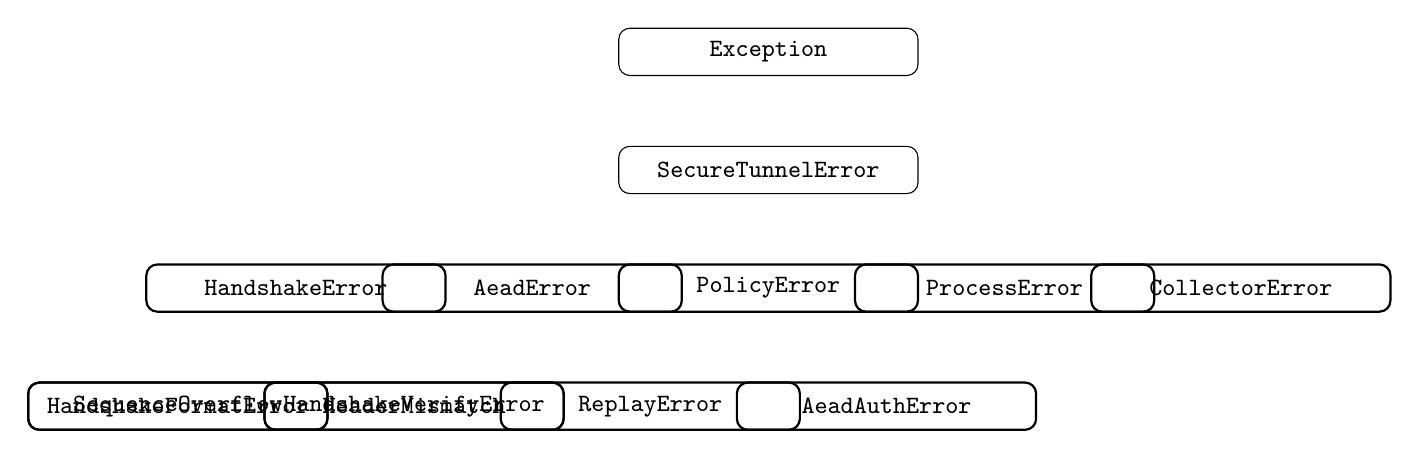
\begin{tikzpicture}[
    node distance=0.6cm and 2.5cm,
    every node/.style={font=\small\ttfamily, draw, rounded corners,
                       minimum width=3.8cm, minimum height=0.6cm},
    edge from parent/.style={->, thick},
    level 1/.style={sibling distance=3cm},
  ]
    \node {Exception}
      child { node {SecureTunnelError}
        child { node {HandshakeError}
          child { node {HandshakeFormatError} }
          child { node {HandshakeVerifyError} }
        }
        child { node {AeadError}
          child { node {SequenceOverflow} }
          child { node {HeaderMismatch} }
          child { node {ReplayError} }
          child { node {AeadAuthError} }
        }
        child { node {PolicyError} }
        child { node {ProcessError} }
        child { node {CollectorError} }
      };
  \end{tikzpicture}
  \caption{Exception class hierarchy.}
  \label{fig:api-exceptions}
\end{figure}

\begin{longtable}{l p{7cm}}
  \caption{Exception classes and their semantics.}
  \label{tab:api-exception-semantics} \\
  \toprule
  \textbf{Exception} & \textbf{When Raised} \\
  \midrule
  \endfirsthead
  \bottomrule
  \endfoot

  \texttt{SecureTunnelError}    & Never raised directly; base for \texttt{except SecureTunnelError} catch-all. \\
  \texttt{HandshakeError}       & Generic handshake failure (timeout, I/O error). \\
  \texttt{HandshakeFormatError} & Wire bytes cannot be parsed (wrong length, bad version). \\
  \texttt{HandshakeVerifyError} & Signature or HMAC verification failed (crypto rejection). \\
  \texttt{AeadError}            & Generic AEAD framing error. \\
  \texttt{SequenceOverflow}     & Sequence counter reached $2^{64}-1$ (must rekey). \\
  \texttt{HeaderMismatch}       & Received header fields do not match local session. \\
  \texttt{ReplayError}          & Sequence number already seen or outside window. \\
  \texttt{AeadAuthError}        & AEAD authentication tag verification failed. \\
  \texttt{PolicyError}          & Policy engine returned invalid decision. \\
  \texttt{ProcessError}         & Managed subprocess crashed or returned non-zero. \\
  \texttt{CollectorError}       & Metric collector failed (permission, timeout, parse). \\
\end{longtable}

% ====================================================================
\section{\texttt{core.aead} --- AEAD Framing Layer}
\label{sec:api-aead}

This is the heart of the data plane.  It handles packet encryption,
decryption, header serialization, nonce derivation, and anti-replay
protection.

\subsection{Constants}

\begin{longtable}{l l p{5cm}}
  \caption{\texttt{core.aead} module constants.}
  \label{tab:api-aead-constants} \\
  \toprule
  \textbf{Name} & \textbf{Value} & \textbf{Purpose} \\
  \midrule
  \endfirsthead
  \bottomrule
  \endfoot

  \texttt{HEADER\_FMT}       & \texttt{"!BBBBB8sQB"} & \texttt{struct} format for the 22-byte packet header. \\
  \texttt{HEADER\_SIZE}      & 22                      & Computed from \texttt{struct.calcsize(HEADER\_FMT)}. \\
  \texttt{TAG\_LEN}          & 16                      & AEAD authentication tag length (bytes). \\
  \texttt{OVERHEAD}          & 38                      & Total per-packet overhead: header + tag. \\
  \texttt{SUPPORTED\_AEADS}  & \texttt{\{"AES-256-GCM", \ldots\}} & Set of algorithm tokens accepted by the framing layer. \\
  \texttt{RETIRED\_AEADS}    & \texttt{\{"AES-128-GCM"\}}        & Algorithms that were once supported but are now rejected. \\
\end{longtable}

\subsection{Class \texttt{AsconAdapter}}
\label{sec:api-ascon-adapter}

An internal adapter that wraps the \texttt{ascon} pure-Python library
to match the interface expected by the \texttt{cryptography} library's
AEAD classes.

\begin{lstlisting}[style=python, caption={AsconAdapter interface}]
class AsconAdapter:
    """AEAD adapter for ASCON-128a (16-byte nonce, 16-byte tag)."""
    
    def __init__(self, key: bytes) -> None:
        """Store the 16-byte symmetric key."""
    
    def encrypt(self, nonce: bytes, data: bytes, aad: bytes) -> bytes:
        """Encrypt `data` with `nonce` and `aad`.
        Returns ciphertext || tag (len = len(data) + 16)."""
    
    def decrypt(self, nonce: bytes, data: bytes, aad: bytes) -> bytes:
        """Decrypt `data` with `nonce` and `aad`.
        Raises AeadAuthError on tag mismatch."""
\end{lstlisting}

\begin{implementationnote}
AsconAdapter is only instantiated when the suite specifies
\texttt{ascon-128a} as the AEAD algorithm.  For AES-256-GCM and
ChaCha20-Poly1305, the \texttt{cryptography} library's native
\texttt{AESGCM} and \texttt{ChaCha20Poly1305} classes are used
directly---they are 50--100$\times$ faster than the pure-Python
ASCON implementation.
\end{implementationnote}

\subsection{Frozen Dataclass \texttt{AeadMeta}}

Immutable metadata identifying a session:

\begin{lstlisting}[style=python, caption={AeadMeta dataclass}]
@dataclass(frozen=True)
class AeadMeta:
    kem_id:    int    # KEM family identifier (1, 3, or 5)
    kem_param: int    # KEM parameter set (1, 2, or 3)
    sig_id:    int    # Signature family identifier
    sig_param: int    # Signature parameter set
\end{lstlisting}

Instances are created once during handshake completion and shared
between the \texttt{Sender} and \texttt{Receiver} objects.

\subsection{Dataclass \texttt{Sender}}

Encrypts plaintext MAVLink packets into \texttt{EncryptedDatagram} wire bytes.

\begin{lstlisting}[style=python, caption={Sender interface}]
@dataclass
class Sender:
    key:        bytes       # 32-byte symmetric key
    meta:       AeadMeta   # Session metadata
    session_id: bytes       # 8-byte session ID
    aead_name:  str         # "AES-256-GCM" | "ChaCha20-Poly1305" | "ascon-128a"
    epoch:      int = 0     # Epoch counter (0-255)
    seq:        int = 0     # Monotonically increasing sequence number
    _cipher:    Any = None  # Lazily initialized AEAD cipher
    
    @property
    def overhead(self) -> int:
        """Return per-packet byte overhead (always 38)."""
    
    def encrypt(self, plaintext: bytes) -> bytes:
        """Encrypt a single MAVLink packet.
        Returns header || ciphertext || tag.
        Raises SequenceOverflow if seq >= 2**64 - 1."""
    
    def reset_epoch(self, new_epoch: int) -> None:
        """Reset the epoch counter and sequence number to zero.
        Used during rekey."""
    
    def stats(self) -> dict:
        """Return a dictionary of sender statistics:
        {'seq': int, 'epoch': int, 'aead': str}."""
\end{lstlisting}

\paragraph{Thread Safety.}
\texttt{Sender} is \textbf{not thread-safe}.  The \texttt{seq} field
is incremented without locking.  In the current architecture this is
acceptable because each proxy instance runs in a single-threaded
\texttt{asyncio} event loop.

\subsection{Dataclass \texttt{Receiver}}

Decrypts \texttt{EncryptedDatagram} wire bytes into plaintext.

\begin{lstlisting}[style=python, caption={Receiver interface}]
@dataclass
class Receiver:
    key:        bytes           # 32-byte symmetric key
    meta:       AeadMeta       # Expected session metadata
    session_id: bytes           # Expected 8-byte session ID
    aead_name:  str             # AEAD algorithm name
    epoch:      int = 0         # Expected epoch
    window:     int = 1024      # Replay window size
    _cipher:    Any = None      # Lazily initialized AEAD cipher
    _high:      int = -1        # Highest accepted sequence number
    _mask:      int = 0         # Bitmask of accepted sequence numbers
    _drop_count: int = 0        # Packets dropped (replay/auth failure)
    
    def decrypt(self, packet: bytes) -> bytes:
        """Decrypt an EncryptedDatagram.
        Performs in order:
          1. Header parsing and version check
          2. Session ID match
          3. KEM/SIG ID match
          4. Anti-replay window check
          5. AEAD decryption and tag verification
        Raises HeaderMismatch, ReplayError, or AeadAuthError."""
    
    def reset_epoch(self, new_epoch: int) -> None:
        """Reset receiver state for a new epoch after rekey."""
    
    def stats(self) -> dict:
        """Return receiver statistics including drop_count and window high."""
    
    def force_accept_seq(self, seq: int) -> None:
        """Force-accept a sequence number without decryption.
        Used in testing only."""
\end{lstlisting}

\subsection{Module Functions}

\begin{longtable}{p{4cm} p{4cm} p{4cm}}
  \caption{\texttt{core.aead} module-level functions.}
  \label{tab:api-aead-functions} \\
  \toprule
  \textbf{Function} & \textbf{Parameters} & \textbf{Returns / Purpose} \\
  \midrule
  \endfirsthead
  \bottomrule
  \endfoot

  \texttt{build\_nonce}   & \texttt{epoch: int, seq: int, nonce\_len: int} & 12- or 16-byte nonce from epoch and sequence number. \\
  \texttt{parse\_header}  & \texttt{data: bytes}                          & Tuple of (version, kem\_id, kem\_param, sig\_id, sig\_param, session\_id, seq, epoch). \\
  \texttt{make\_sender\_receiver} & \texttt{key\_d2g, key\_g2d, meta, session\_id, aead\_name, mode} & Returns \texttt{(Sender, Receiver)} pair with correct key assignment based on mode ("drone" or "gcs"). \\
\end{longtable}

% ====================================================================
\section{\texttt{core.handshake} --- Wire Format Serialization}
\label{sec:api-handshake}

\subsection{Frozen Dataclass \texttt{ServerHelloData}}

\begin{lstlisting}[style=python, caption={ServerHelloData fields}]
@dataclass(frozen=True)
class ServerHelloData:
    version:      int     # Wire protocol version (1)
    kem_name:     str     # OQS KEM algorithm name
    sig_name:     str     # OQS signature algorithm name
    session_id:   bytes   # 8-byte random session ID
    challenge:    bytes   # 8-byte freshness nonce
    kem_pk:       bytes   # KEM public key bytes
\end{lstlisting}

\subsection{Class \texttt{HandshakeSerializer}}

\begin{lstlisting}[style=python, caption={HandshakeSerializer interface}]
class HandshakeSerializer:
    @staticmethod
    def build_transcript(data: ServerHelloData) -> bytes:
        """Build the signable transcript from ServerHello fields.
        Returns: version || b"pq-drone-gcs:v1" || session_id || 
                 kem_name || sig_name || kem_pk || challenge"""
    
    @staticmethod
    def serialize_server_hello(
        data: ServerHelloData, signature: bytes
    ) -> bytes:
        """Serialize ServerHello + signature to wire bytes.
        Format: see Table 22.1."""
    
    @staticmethod
    def deserialize_server_hello(
        raw: bytes
    ) -> tuple[ServerHelloData, bytes]:
        """Parse wire bytes into (ServerHelloData, signature).
        Raises HandshakeFormatError on malformed input."""
\end{lstlisting}

\subsection{Module Functions}

\begin{longtable}{p{4.5cm} p{3.5cm} p{4.5cm}}
  \caption{\texttt{core.handshake} module-level functions.}
  \label{tab:api-handshake-functions} \\
  \toprule
  \textbf{Function} & \textbf{Parameters} & \textbf{Returns} \\
  \midrule
  \endfirsthead
  \bottomrule
  \endfoot

  \texttt{generate\_session\_id} & (none) & 8 random bytes from \texttt{os.urandom}. \\
  \texttt{generate\_challenge} & (none) & 8 random bytes from \texttt{os.urandom}. \\
  \texttt{compute\_hmac}  & \texttt{psk: bytes, data: bytes} & 32-byte HMAC-SHA256 tag. \\
  \texttt{verify\_hmac}   & \texttt{psk, data, tag} & \texttt{bool} (constant-time comparison). \\
  \texttt{build\_server\_hello} & \texttt{kem\_name, sig\_name, kem\_pk} & \texttt{ServerHelloData} with random IDs. \\
  \texttt{serialize\_client\_reply} & \texttt{kem\_ct: bytes, hmac\_tag: bytes} & Wire bytes for ClientReply. \\
\end{longtable}

% ====================================================================
\section{\texttt{core.crypto\_utils} --- Cryptographic Primitives}
\label{sec:api-crypto-utils}

This module wraps the Open Quantum Safe (OQS) library and the
Python \texttt{cryptography} library to provide high-level
cryptographic operations.

\subsection{Frozen Dataclass \texttt{CryptoResult}}

\begin{lstlisting}[style=python, caption={CryptoResult fields}]
@dataclass(frozen=True)
class CryptoResult:
    shared_secret: bytes    # KEM shared secret (32 or 64 bytes)
    ciphertext:    bytes    # KEM ciphertext
    kem_name:      str      # Algorithm used
    sig_name:      str      # Signature algorithm
    session_id:    bytes    # Session identifier
    key_d2g:       bytes    # Derived drone-to-GCS key (32 bytes)
    key_g2d:       bytes    # Derived GCS-to-drone key (32 bytes)
    elapsed_ms:    float    # Total handshake time
\end{lstlisting}

\subsection{Key Derivation}

\begin{lstlisting}[style=python, caption={HKDF key derivation}]
def derive_keys(
    shared_secret: bytes,
    session_id:    bytes,
    kem_name:      str,
    sig_name:      str,
) -> tuple[bytes, bytes]:
    """Derive two 32-byte directional keys from the KEM shared secret.
    
    Uses HKDF-SHA256 with:
      salt = b"pq-drone-gcs|hkdf|v1"
      info = b"pq-drone-gcs:kdf:v1|" + session_id + b"|" + kem_name + b"|" + sig_name
      length = 64 bytes
    
    Returns (key_d2g, key_g2d) = OKM[0:32], OKM[32:64].
    """
\end{lstlisting}

\subsection{OQS Wrappers}

\begin{longtable}{p{4cm} p{4cm} p{4.5cm}}
  \caption{\texttt{core.crypto\_utils} OQS wrapper functions.}
  \label{tab:api-crypto-oqs} \\
  \toprule
  \textbf{Function} & \textbf{Parameters} & \textbf{Returns / Purpose} \\
  \midrule
  \endfirsthead
  \bottomrule
  \endfoot

  \texttt{kem\_keygen}     & \texttt{kem\_name: str}                 & \texttt{(public\_key, secret\_key)} tuple. Wraps \texttt{oqs.KeyEncapsulation}. \\
  \texttt{kem\_encapsulate} & \texttt{kem\_name, public\_key}        & \texttt{(ciphertext, shared\_secret)} tuple. \\
  \texttt{kem\_decapsulate} & \texttt{kem\_name, ciphertext, secret\_key} & \texttt{shared\_secret} bytes. \\
  \texttt{sig\_keygen}      & \texttt{sig\_name: str}                & \texttt{(public\_key, secret\_key)} tuple. Wraps \texttt{oqs.Signature}. \\
  \texttt{sig\_sign}        & \texttt{sig\_name, message, secret\_key} & \texttt{signature} bytes. \\
  \texttt{sig\_verify}      & \texttt{sig\_name, message, signature, public\_key} & \texttt{bool} (True if valid). \\
  \texttt{get\_kem\_details} & \texttt{kem\_name: str}               & Dict with \texttt{pk\_len}, \texttt{sk\_len}, \texttt{ct\_len}, \texttt{ss\_len}. \\
  \texttt{get\_sig\_details} & \texttt{sig\_name: str}               & Dict with \texttt{pk\_len}, \texttt{sk\_len}, \texttt{sig\_len}. \\
  \texttt{list\_available\_kems} & (none)                            & List of KEM names supported by installed OQS. \\
  \texttt{list\_available\_sigs} & (none)                            & List of signature names supported by installed OQS. \\
\end{longtable}

\begin{securitynote}
All OQS wrapper functions perform algorithm name validation before
calling into the C library.  An unrecognised algorithm name raises
\texttt{ValueError} immediately, preventing injection of unsupported
algorithm strings through configuration.
\end{securitynote}

% ====================================================================
\section{\texttt{core.rate\_limiter} --- Token Bucket Rate Limiter}
\label{sec:api-rate-limiter}

The rate limiter protects the TCP handshake endpoint from
denial-of-service attacks by limiting the number of handshakes
accepted per unit time.

\begin{lstlisting}[style=python, caption={TokenBucketRateLimiter interface}]
class TokenBucketRateLimiter:
    def __init__(
        self,
        capacity:   int   = 5,     # Maximum burst size
        refill_rate: float = 3.0,  # Tokens per second
    ) -> None:
        """Create a token bucket with given capacity and refill rate."""
    
    def try_acquire(self) -> bool:
        """Attempt to acquire one token.
        Returns True if a token was available, False otherwise.
        Thread-safe (uses monotonic clock, no mutex needed for
        single-threaded asyncio)."""
    
    def tokens_available(self) -> float:
        """Return the current (fractional) number of tokens."""
    
    def time_until_available(self) -> float:
        """Seconds until at least one token is available.
        Returns 0.0 if tokens are currently available."""
    
    def reset(self) -> None:
        """Reset the bucket to full capacity."""
    
    @property
    def capacity(self) -> int:
        """Maximum tokens in the bucket."""
    
    @property
    def refill_rate(self) -> float:
        """Tokens added per second."""
    
    def stats(self) -> dict:
        """Return {'tokens': float, 'capacity': int, 
                   'refill_rate': float, 'total_acquired': int,
                   'total_rejected': int}."""
\end{lstlisting}

\paragraph{Algorithm.}
The token bucket uses a lazy-evaluation approach:

\begin{enumerate}
  \item On each \texttt{try\_acquire()} call, compute elapsed time since
        last refill: $\Delta t = t_{\text{now}} - t_{\text{last}}$.
  \item Add $\Delta t \times \text{refill\_rate}$ tokens, capped at
        \texttt{capacity}.
  \item If tokens $\geq 1$, decrement by 1 and return True.
  \item Otherwise, return False.
\end{enumerate}

This avoids background threads or timers.

% ====================================================================
\section{\texttt{core.config} --- Centralised Configuration}
\label{sec:api-config}

\subsection{The \texttt{CONFIG} Dictionary}

All runtime configuration is stored in a single module-level dictionary
\texttt{CONFIG} with approximately 100~keys, organised into groups:

\begin{longtable}{l p{8cm}}
  \caption{\texttt{CONFIG} key groups.}
  \label{tab:api-config-groups} \\
  \toprule
  \textbf{Group} & \textbf{Key Prefix / Description} \\
  \midrule
  \endfirsthead
  \bottomrule
  \endfoot

  Network        & \texttt{TCP\_PORT}, \texttt{UDP\_IN\_PORT}, \texttt{UDP\_OUT\_PORT},
                   \texttt{GCS\_HOST}, \texttt{DRONE\_HOST} --- socket addresses. \\
  Cryptography   & \texttt{KEM\_ALG}, \texttt{SIG\_ALG}, \texttt{AEAD\_ALG},
                   \texttt{DRONE\_PSK} --- algorithm selection and pre-shared key. \\
  Keys           & \texttt{GCS\_SIG\_PRIVATE\_KEY}, \texttt{GCS\_SIG\_PUBLIC\_KEY},
                   \texttt{KEY\_DIR} --- file paths for cryptographic keys. \\
  Security       & \texttt{STRICT\_UDP\_PEER\_MATCH}, \texttt{REPLAY\_WINDOW},
                   \texttt{RATE\_LIMIT\_*} --- security policy knobs. \\
  Timeouts       & \texttt{HANDSHAKE\_TIMEOUT}, \texttt{PROXY\_IDLE\_TIMEOUT},
                   \texttt{HEALTH\_CHECK\_INTERVAL} --- timing parameters. \\
  Benchmark      & \texttt{BENCHMARK.*} --- nested dict for benchmark pipeline
                   configuration (iterations, suite list, output paths). \\
  Automation     & \texttt{AUTO\_DRONE.*}, \texttt{AUTO\_GCS.*} --- nested dicts
                   for automated end-to-end testing. \\
  Scheduler      & \texttt{SCHEDULER\_*} --- suite rotation policy parameters
                   (time per suite, overlap window, ramp-up). \\
  QoS            & \texttt{UDP\_DSCP\_VALUE}, \texttt{UDP\_BUFFER\_SIZE} ---
                   Quality of Service and socket buffer tuning. \\
\end{longtable}

\subsection{Environment Variable Override}

\begin{lstlisting}[style=python, caption={Environment variable override mechanism}]
def apply_env_overrides() -> list[str]:
    """Scan os.environ for keys prefixed with SECDRONE_.
    For each match:
      1. Strip the SECDRONE_ prefix
      2. Look up the key in CONFIG
      3. Cast the env value to the expected type
      4. Override CONFIG[key]
    Returns a list of overridden key names (for logging).
    """

def validate_config() -> list[str]:
    """Validate all CONFIG values.
    Checks:
      - Required keys are present and non-empty
      - Port numbers are in range 1024-65535
      - PSK is valid base64 and decodes to >= 32 bytes
      - Key file paths exist and have correct permissions
      - Algorithm names are recognised by OQS
    Returns a list of validation warnings (empty = all OK).
    """
\end{lstlisting}

% ====================================================================
\section{\texttt{core.suites} --- Cipher Suite Management}
\label{sec:api-suites}

\subsection{Suite Generation}

The \texttt{suites} module defines the universe of valid cipher suites
by computing the Cartesian product of KEM, AEAD, and signature algorithms.

\begin{lstlisting}[style=python, caption={Suite generation constants}]
SUPPORTED_KEMS = [
    "ML-KEM-512", "ML-KEM-768", "ML-KEM-1024",
    "HQC-128", "HQC-192", "HQC-256",
    "Classic-McEliece-348864", "Classic-McEliece-460896",
    "Classic-McEliece-8192128",
]

SUPPORTED_SIGS = [
    "ML-DSA-44", "ML-DSA-65", "ML-DSA-87",
    "Falcon-512", "Falcon-1024",
    "SPHINCS+-SHA2-128f-simple", "SPHINCS+-SHA2-192f-simple",
    "SPHINCS+-SHA2-256f-simple",
]

SUPPORTED_AEADS = [
    "AES-256-GCM", "ChaCha20-Poly1305", "ascon-128a",
]

# ALL_SUITES: OrderedDict[str, SuiteConfig]
# Generated as: product(KEMS, AEADS, SIGS) -> 9 * 3 * 8 = 216 suites
\end{lstlisting}

\subsection{Suite Identifier Format}

Each suite has a canonical string identifier:
\begin{center}
  \texttt{cs-\{kem\}-\{aead\}-\{sig\}}
\end{center}

Examples:
\begin{itemize}
  \item \texttt{cs-mlkem768-aesgcm-mldsa65}
  \item \texttt{cs-mceliece348864-chacha-falcon512}
  \item \texttt{cs-hqc256-ascon128a-sphincssha2256fsimple}
\end{itemize}

\subsection{Module Functions}

\begin{longtable}{p{4cm} p{3.5cm} p{5cm}}
  \caption{\texttt{core.suites} module-level functions.}
  \label{tab:api-suites-functions} \\
  \toprule
  \textbf{Function} & \textbf{Parameters} & \textbf{Returns / Purpose} \\
  \midrule
  \endfirsthead
  \bottomrule
  \endfoot

  \texttt{get\_suite}        & \texttt{suite\_id: str}         & \texttt{SuiteConfig} or raises \texttt{KeyError}. \\
  \texttt{list\_suites}      & \texttt{kem\_filter, sig\_filter, aead\_filter} & Filtered list of suite IDs. \\
  \texttt{list\_fast\_suites} & (none)                         & Suites using ML-KEM only (fast handshakes). \\
  \texttt{suite\_to\_ids}    & \texttt{suite\_id: str}         & \texttt{AeadMeta} tuple for header encoding. \\
  \texttt{ids\_to\_suite}    & \texttt{kem\_id, kem\_param, sig\_id, sig\_param} & Reverse lookup: IDs $\to$ suite ID string. \\
  \texttt{validate\_suite}   & \texttt{suite\_id: str}         & \texttt{bool} + error message if invalid. \\
  \texttt{group\_by\_kem}    & (none)                          & Dict mapping KEM name $\to$ list of suite IDs. \\
  \texttt{group\_by\_sig}    & (none)                          & Dict mapping SIG name $\to$ list of suite IDs. \\
  \texttt{group\_by\_aead}   & (none)                          & Dict mapping AEAD name $\to$ list of suite IDs. \\
  \texttt{generate\_keys\_for\_suite} & \texttt{suite\_id, key\_dir} & Generate and save KEM+SIG keypairs. \\
  \texttt{count\_suites}     & (none)                          & Total number of defined suites (216). \\
  \texttt{get\_suite\_security\_level} & \texttt{suite\_id}    & Minimum NIST security level (1, 3, or 5). \\
  \texttt{estimate\_handshake\_ms} & \texttt{suite\_id}        & Estimated handshake time from algorithm benchmarks. \\
  \texttt{estimate\_throughput\_mbps} & \texttt{suite\_id}     & Estimated AEAD throughput from algorithm benchmarks. \\
  \texttt{sort\_by\_handshake\_time} & \texttt{suite\_ids}     & Sort suite list by estimated handshake speed. \\
  \texttt{filter\_by\_level} & \texttt{min\_level: int}        & Suites with security level $\geq$ min\_level. \\
  \texttt{get\_all\_kem\_names} & (none)                       & Deduplicated list of KEM algorithm names. \\
  \texttt{get\_all\_sig\_names} & (none)                       & Deduplicated list of SIG algorithm names. \\
\end{longtable}

% ====================================================================
\section{\texttt{core.keys} --- Key Pair Management}
\label{sec:api-keys}

\subsection{Dataclass \texttt{KeyPairInfo}}

\begin{lstlisting}[style=python, caption={KeyPairInfo dataclass}]
@dataclass
class KeyPairInfo:
    algorithm:    str       # OQS algorithm name
    pk_path:      Path      # Public key file path
    sk_path:      Path      # Secret key file path
    pk_bytes:     int       # Public key size in bytes
    sk_bytes:     int       # Secret key size in bytes
    pk_hash:      str       # SHA-256 hex digest of public key
    sk_hash:      str       # SHA-256 hex digest of secret key
    created_at:   str       # ISO 8601 creation timestamp
    fingerprint:  str       # First 16 hex chars of pk_hash
    nist_level:   int       # NIST security level (1, 3, or 5)
    key_type:     str       # "kem" or "sig"
    format_ver:   int       # Key file format version (1)
    metadata:     dict      # Additional metadata (OQS version, etc.)
\end{lstlisting}

\subsection{Dataclass \texttt{KeyBundle}}

\begin{lstlisting}[style=python, caption={KeyBundle dataclass}]
@dataclass
class KeyBundle:
    kem:  KeyPairInfo    # KEM key pair metadata
    sig:  KeyPairInfo    # Signature key pair metadata
    suite_id: str        # Associated cipher suite ID
\end{lstlisting}

\subsection{Module Functions}

\begin{longtable}{p{4cm} p{3.5cm} p{5cm}}
  \caption{\texttt{core.keys} module-level functions.}
  \label{tab:api-keys-functions} \\
  \toprule
  \textbf{Function} & \textbf{Parameters} & \textbf{Returns / Purpose} \\
  \midrule
  \endfirsthead
  \bottomrule
  \endfoot

  \texttt{save\_key\_pair}  & \texttt{pk, sk, alg, key\_dir, key\_type} & Writes .pub and .key files with metadata header. \\
  \texttt{load\_public\_key} & \texttt{path: Path}              & Raw public key bytes. \\
  \texttt{load\_secret\_key} & \texttt{path: Path}              & Raw secret key bytes. \\
  \texttt{load\_key\_pair}   & \texttt{pk\_path, sk\_path}      & \texttt{(pk\_bytes, sk\_bytes)} tuple. \\
  \texttt{key\_info}         & \texttt{path: Path}              & \texttt{KeyPairInfo} from file metadata. \\
  \texttt{generate\_and\_save} & \texttt{alg, key\_dir, key\_type} & Generate keys and save; return \texttt{KeyPairInfo}. \\
  \texttt{rotate\_keys}      & \texttt{suite\_id, key\_dir}     & Generate new keys, archive old ones, return new bundle. \\
  \texttt{verify\_key\_integrity} & \texttt{path: Path}         & Check SHA-256 hash matches metadata; return bool. \\
  \texttt{list\_key\_files}  & \texttt{key\_dir: Path}           & List all .pub and .key files with metadata. \\
  \texttt{export\_public\_keys} & \texttt{key\_dir, output\_dir} & Copy all .pub files to output directory. \\
  \texttt{import\_public\_key} & \texttt{source, key\_dir}       & Copy external public key into key directory. \\
\end{longtable}

% ====================================================================
\section{\texttt{core.proxy} --- Proxy Engine}
\label{sec:api-proxy}

The proxy module contains the main event loop and is the largest
module in the codebase (1{,}665~lines).

\subsection{Class \texttt{ProxyEngine}}

\begin{lstlisting}[style=python, caption={ProxyEngine class outline}]
class ProxyEngine:
    def __init__(
        self,
        config:     dict,
        mode:       str,          # "drone" or "gcs"
        suite_id:   str,
        key_dir:    Path,
        sig_pub:    Path | None = None,
        sig_priv:   Path | None = None,
    ) -> None:
        """Initialise the proxy with configuration and key paths.
        Does NOT start any I/O (call run() for that)."""
    
    async def run(self) -> None:
        """Main entry point. Performs:
          1. TCP handshake (server or client based on mode)
          2. Key derivation
          3. UDP event loop (encrypt/decrypt)
          4. Rekey when triggered
          5. Cleanup on exit"""
    
    async def perform_handshake(self) -> CryptoResult:
        """Execute the 1-RTT PQC handshake.
        GCS mode: listen -> accept -> keygen -> sign -> send -> recv -> verify -> decap
        Drone mode: connect -> recv -> verify -> encap -> hmac -> send"""
    
    async def data_loop(self) -> None:
        """Bidirectional UDP encrypt/decrypt event loop.
        Uses asyncio.DatagramProtocol under the hood."""
    
    async def rekey(self) -> None:
        """Initiate a rekey: pause data loop, new handshake, derive new keys,
        resume data loop with new Sender/Receiver."""
    
    def stop(self) -> None:
        """Signal the proxy to shut down gracefully.
        Closes all sockets, releases key material."""
    
    @property
    def is_running(self) -> bool:
        """True if the proxy event loop is active."""
\end{lstlisting}

\paragraph{Instance Variables (Security-Critical).}

\begin{longtable}{l l p{5cm}}
  \caption{Security-critical instance variables of \texttt{ProxyEngine}.}
  \label{tab:api-proxy-instance-vars} \\
  \toprule
  \textbf{Variable} & \textbf{Type} & \textbf{Security Role} \\
  \midrule
  \endfirsthead
  \bottomrule
  \endfoot

  \texttt{\_sender}       & \texttt{Sender}          & Holds the encryption key; zeroed on stop/rekey. \\
  \texttt{\_receiver}     & \texttt{Receiver}        & Holds the decryption key; zeroed on stop/rekey. \\
  \texttt{\_psk}          & \texttt{bytes}           & Pre-shared key for HMAC; loaded once, never logged. \\
  \texttt{\_sig\_sk}      & \texttt{bytes}           & Signature secret key (GCS only); loaded from file. \\
  \texttt{\_sig\_pk}      & \texttt{bytes}           & Signature public key (both sides). \\
  \texttt{\_session\_id}  & \texttt{bytes}           & 8-byte session ID; changes on rekey. \\
  \texttt{\_rate\_limiter} & \texttt{TokenBucketRateLimiter} & Protects handshake from DoS. \\
  \texttt{\_tcp\_sock}    & \texttt{socket}          & TCP socket for handshake; closed after use. \\
  \texttt{\_udp\_sock}    & \texttt{socket}          & UDP socket for data plane. \\
  \texttt{\_rekey\_event} & \texttt{asyncio.Event}   & Signals rekey request. \\
\end{longtable}

\subsection{Class \texttt{DatagramProtocol}}

Internal \texttt{asyncio.DatagramProtocol} subclass used by the proxy
for non-blocking UDP I/O:

\begin{lstlisting}[style=python, caption={DatagramProtocol outline}]
class _TunnelDatagramProtocol(asyncio.DatagramProtocol):
    def __init__(self, receiver: Receiver, callback) -> None: ...
    def datagram_received(self, data: bytes, addr: tuple) -> None:
        """Called by asyncio for each incoming UDP packet.
        Decrypts, validates, and forwards to callback."""
    def error_received(self, exc: Exception) -> None:
        """Handle UDP errors (logged, not fatal)."""
    def connection_lost(self, exc) -> None:
        """Socket closed (normal or error)."""
\end{lstlisting}

\subsection{Module Functions}

\begin{longtable}{p{4cm} p{3.5cm} p{5cm}}
  \caption{\texttt{core.proxy} module-level functions.}
  \label{tab:api-proxy-functions} \\
  \toprule
  \textbf{Function} & \textbf{Parameters} & \textbf{Returns / Purpose} \\
  \midrule
  \endfirsthead
  \bottomrule
  \endfoot

  \texttt{dscp\_to\_tos}       & \texttt{dscp: int}      & TOS byte value ($\text{dscp} \ll 2$). \\
  \texttt{parse\_aead\_header}  & \texttt{data: bytes}    & Parsed header fields tuple. \\
  \texttt{validate\_proxy\_config} & \texttt{config: dict} & Raise on invalid config. \\
  \texttt{full\_handshake}      & \texttt{mode, config, ...} & Complete 1-RTT handshake; returns \texttt{CryptoResult}. \\
  \texttt{create\_udp\_socket}  & \texttt{host, port, dscp} & Configured UDP socket (SO\_REUSEADDR, DSCP, buffer). \\
  \texttt{suite\_to\_ids}       & \texttt{suite\_id}      & \texttt{AeadMeta} for the suite. \\
  \texttt{build\_sender\_receiver} & \texttt{result, mode, aead\_name} & \texttt{(Sender, Receiver)} pair. \\
  \texttt{interactive\_rekey\_console} & \texttt{engine: ProxyEngine} & Stdin listener for manual rekey ("r" + Enter). \\
  \texttt{run\_proxy}           & \texttt{mode, suite\_id, ...} & \textbf{Main entry point}: creates ProxyEngine and calls \texttt{run()}. \\
\end{longtable}

% ====================================================================
\section{\texttt{core.metrics\_schema} --- Metrics Dataclasses}
\label{sec:api-metrics-schema}

The metrics schema defines 18~dataclass categories (A through R)
plus an aggregator class.  Each category corresponds to a specific
aspect of the system being benchmarked.

\begin{longtable}{c l r p{4.5cm}}
  \caption{Metrics schema categories overview.}
  \label{tab:api-metrics-categories} \\
  \toprule
  \textbf{Cat.} & \textbf{Class Name} & \textbf{Fields} & \textbf{Coverage} \\
  \midrule
  \endfirsthead
  \toprule
  \textbf{Cat.} & \textbf{Class Name} & \textbf{Fields} & \textbf{Coverage} \\
  \midrule
  \endhead
  \bottomrule
  \endfoot

  A & \texttt{EnvironmentMetrics}   & 12 & Host OS, kernel, CPU model, RAM, Python version, OQS version, date. \\
  B & \texttt{HandshakeMetrics}     & 10 & KEM keygen/encap/decap times, SIG sign/verify times, total time, round-trips. \\
  C & \texttt{SessionMetrics}       & 8  & Session duration, bytes encrypted/decrypted, packets tx/rx, uptime ratio. \\
  D & \texttt{LatencyMetrics}       & 8  & End-to-end latency (min/max/avg/p50/p95/p99), jitter, measurement count. \\
  E & \texttt{ArtifactMetrics}      & 10 & Public key size, ciphertext size, signature size, shared secret size, nonce size, total wire. \\
  F & \texttt{ThroughputMetrics}    & 6  & Encrypt MB/s, decrypt MB/s, packets per second (encrypt/decrypt), aggregate. \\
  G & \texttt{OverheadMetrics}      & 6  & Header overhead bytes, tag overhead bytes, expansion ratio, bandwidth efficiency. \\
  H & \texttt{ValidationMetrics}    & 8  & Signature valid flag, HMAC valid flag, AEAD tests passed, replay tests, CRC checks. \\
  I & \texttt{MAVDroneMetrics}      & 8  & MAVProxy drone-side: tx/rx packets per second, heartbeat rate, command ack rate. \\
  J & \texttt{MAVGCSMetrics}        & 6  & MAVProxy GCS-side: total messages, sequence gaps, dedup count. \\
  K & \texttt{ErrorMetrics}         & 8  & CRC errors, decode errors, drops, duplicates, out-of-order, auth failures. \\
  L & \texttt{FlightControlMetrics} & 8  & FC mode, armed state, battery voltage, attitude rate, position rate. \\
  M & \texttt{SchedulerMetrics}     & 6  & Tick interval, policy name, policy state, suite index, total suites. \\
  N & \texttt{DroneSystemMetrics}   & 8  & CPU usage, memory usage, temperature, load averages (1/5/15 min). \\
  O & \texttt{GCSSystemMetrics}     & 8  & Same as N but for the GCS host. \\
  P & \texttt{PowerMetrics}         & 6  & Average power (W), total energy (J), energy per handshake (J). \\
  Q & \texttt{SamplingMetrics}      & 4  & Sample count, sampling rate (Hz), collection duration (s). \\
  R & \texttt{ValidationSummary}    & 8  & Expected/collected/lost samples, success rate, pass/fail, metric status map. \\
\end{longtable}

\subsection{Aggregator Class \texttt{BenchmarkRecord}}

\begin{lstlisting}[style=python, caption={BenchmarkRecord aggregator}]
@dataclass
class BenchmarkRecord:
    suite_id:    str
    suite_index: int
    timestamp:   str             # ISO 8601 UTC
    elapsed_s:   float
    categories:  dict[str, Any]  # {"A": EnvironmentMetrics, ...}
    
    def to_dict(self) -> dict:
        """Serialise to JSON-compatible dict (recursive dataclass -> dict)."""
    
    @classmethod
    def from_dict(cls, d: dict) -> 'BenchmarkRecord':
        """Deserialise from dict (e.g., from JSONL line)."""
    
    def validate(self) -> list[str]:
        """Check all categories present; return list of warnings."""
    
    def to_jsonl_line(self) -> str:
        """Serialise to a single JSONL line (no trailing newline)."""
    
    @classmethod
    def from_jsonl_line(cls, line: str) -> 'BenchmarkRecord':
        """Parse a JSONL line into a BenchmarkRecord."""
    
    def merge(self, other: 'BenchmarkRecord') -> 'BenchmarkRecord':
        """Merge two records (for multi-run aggregation)."""
\end{lstlisting}

% ====================================================================
\section{\texttt{core.collectors} --- Metric Collectors}
\label{sec:api-collectors}

Collectors are responsible for gathering runtime data from various
system sources.

\subsection{Class \texttt{SystemCollector}}

\begin{lstlisting}[style=python, caption={SystemCollector interface}]
class SystemCollector:
    """Collects host-level metrics (CPU, RAM, temperature, load)."""
    
    def __init__(self, role: str = "drone") -> None:
        """role: 'drone' or 'gcs'."""
    
    def collect(self) -> dict:
        """Snapshot current system metrics.
        Returns dict with keys: cpu_percent, memory_percent,
        temperature_c, load_1m, load_5m, load_15m."""
    
    def collect_averaged(self, samples: int = 5, interval: float = 0.5) -> dict:
        """Take multiple samples and return averaged metrics."""
    
    def is_available(self) -> bool:
        """True if the collector can access required system interfaces.
        (e.g., /sys/class/thermal on Linux, WMI on Windows)."""
\end{lstlisting}

\subsection{Class \texttt{ProcessCollector}}

\begin{lstlisting}[style=python, caption={ProcessCollector interface}]
class ProcessCollector:
    """Collects per-process metrics using psutil."""
    
    def collect_for_pid(self, pid: int) -> dict:
        """Collect CPU and memory stats for a specific PID.
        Returns dict with: cpu_percent, memory_rss_mb, 
        memory_vms_mb, num_threads, num_fds."""
    
    def collect_for_name(self, name: str) -> dict:
        """Find process by name and collect metrics."""
    
    def collect_children(self, parent_pid: int) -> list[dict]:
        """Collect metrics for all child processes."""
    
    def is_running(self, pid: int) -> bool:
        """Check if PID exists and is alive."""
\end{lstlisting}

\subsection{Class \texttt{MAVLinkCollector}}

\begin{lstlisting}[style=python, caption={MAVLinkCollector interface}]
class MAVLinkCollector:
    """Parses MAVProxy log output for message statistics."""
    
    def parse_log(self, log_path: Path) -> dict:
        """Parse MAVProxy log file for msg counts, rates, errors.
        Returns dict with: total_messages, heartbeat_count,
        command_ack_count, crc_errors, seq_gaps, msg_types."""
    
    def parse_realtime(self, line: str) -> dict | None:
        """Parse a single MAVProxy log line.
        Returns metric dict or None if line is not a metric."""
    
    def aggregate(self, samples: list[dict]) -> dict:
        """Aggregate multiple samples into summary statistics."""
\end{lstlisting}

\subsection{Class \texttt{LatencyCollector}}

\begin{lstlisting}[style=python, caption={LatencyCollector interface}]
class LatencyCollector:
    """Collects end-to-end latency measurements."""
    
    def __init__(self, max_samples: int = 10000) -> None:
        """Circular buffer with configurable max size."""
    
    def record(self, latency_ms: float) -> None:
        """Record a single latency sample."""
    
    def stats(self) -> dict:
        """Compute statistics: min, max, mean, median,
        p95, p99, stddev, count, jitter."""
    
    def reset(self) -> None:
        """Clear all recorded samples."""
    
    def histogram(self, bins: int = 50) -> list[tuple[float, int]]:
        """Return histogram data: (bin_center, count) pairs."""
\end{lstlisting}

\subsection{Class \texttt{ThroughputCollector}}

\begin{lstlisting}[style=python, caption={ThroughputCollector interface}]
class ThroughputCollector:
    """Tracks bytes and packets over time for throughput calculation."""
    
    def __init__(self) -> None:
        """Initialise counters to zero."""
    
    def record_encrypt(self, plaintext_bytes: int) -> None:
        """Record an encrypt operation."""
    
    def record_decrypt(self, ciphertext_bytes: int) -> None:
        """Record a decrypt operation."""
    
    def stats(self) -> dict:
        """Compute throughput: encrypt_mbps, decrypt_mbps,
        encrypt_pps, decrypt_pps, total_bytes."""
    
    def reset(self) -> None:
        """Zero all counters and reset timestamp."""
\end{lstlisting}

\subsection{Class \texttt{PowerCollector}}

\begin{lstlisting}[style=python, caption={PowerCollector interface}]
class PowerCollector:
    """Reads power sensor data (platform-specific)."""
    
    def __init__(self, sensor_path: str = "/sys/class/power_supply") -> None:
        """Specify power sensor sysfs path."""
    
    def is_available(self) -> bool:
        """True if power sensors are accessible."""
    
    def sample(self) -> dict:
        """Take a single power reading.
        Returns: voltage_v, current_a, power_w."""
    
    def integrate(self, duration_s: float, interval: float = 0.1) -> dict:
        """Integrate power over duration.
        Returns: avg_power_w, total_energy_j, peak_power_w."""
\end{lstlisting}

% ====================================================================
\section{\texttt{core.runner} --- Proxy Lifecycle Management}
\label{sec:api-runner}

The runner module manages proxy and MAVProxy as external processes.

\subsection{Class \texttt{ProxyRunner}}

\begin{lstlisting}[style=python, caption={ProxyRunner interface (abbreviated)}]
class ProxyRunner:
    """Manages proxy as a subprocess with health monitoring."""
    
    def __init__(self, config: dict, mode: str, suite_id: str) -> None:
        """Configure but do not start."""
    
    async def start(self) -> None:
        """Start the proxy subprocess.
        Waits for 'handshake complete' log line."""
    
    async def stop(self, timeout: float = 10.0) -> None:
        """Graceful stop: SIGTERM, wait, SIGKILL if needed."""
    
    async def restart(self) -> None:
        """Stop then start."""
    
    async def wait_healthy(self, timeout: float = 30.0) -> bool:
        """Block until proxy reports healthy or timeout."""
    
    def is_alive(self) -> bool:
        """Check if subprocess is running."""
    
    @property
    def pid(self) -> int | None:
        """PID of subprocess, or None if not running."""
    
    def logs(self, tail: int = 50) -> list[str]:
        """Return last N lines of subprocess output."""
    
    # ... 12 more methods for health checks, metrics, etc.
\end{lstlisting}

% ====================================================================
\section{\texttt{core.process\_mgr} --- Process Manager}
\label{sec:api-process-mgr}

\subsection{Dataclasses}

\begin{lstlisting}[style=python, caption={Process manager dataclasses}]
@dataclass
class ProcessConfig:
    command:      list[str]    # Command and arguments
    name:         str          # Human-readable process name
    cwd:          Path         # Working directory
    env:          dict         # Environment variables
    
@dataclass
class ProcessState:
    pid:          int | None
    return_code:  int | None
    started_at:   float | None
    stopped_at:   float | None
    restart_count: int
    last_health:  bool
    stdout_lines: list[str]
    stderr_lines: list[str]
    status:       str        # "stopped" | "starting" | "running" | "failed"
    health_checks_passed: int
    health_checks_failed: int
\end{lstlisting}

\subsection{Protocol \texttt{HealthChecker}}

\begin{lstlisting}[style=python, caption={HealthChecker protocol}]
class HealthChecker(Protocol):
    def check(self, state: ProcessState) -> bool: ...
    def reset(self) -> None: ...
    def interval_seconds(self) -> float: ...
    def describe(self) -> str: ...
\end{lstlisting}

Four implementations are provided:

\begin{longtable}{l p{7cm}}
  \caption{HealthChecker implementations.}
  \label{tab:api-health-checkers} \\
  \toprule
  \textbf{Class} & \textbf{Strategy} \\
  \midrule
  \endfirsthead
  \bottomrule
  \endfoot

  \texttt{PidHealthChecker}     & Checks \texttt{os.kill(pid, 0)} succeeds (process exists). \\
  \texttt{LogHealthChecker}     & Scans stdout for a success pattern (e.g.\ ``handshake complete'').
    Static method \texttt{for\_proxy()} returns checker configured for proxy. \\
  \texttt{TcpHealthChecker}     & Attempts TCP connect to a port; success = healthy. \\
  \texttt{CompositeHealthChecker} & Logical AND of multiple checkers; all must pass. \\
\end{longtable}

\subsection{Factory Function}

\begin{lstlisting}[style=python, caption={Process manager factory}]
def create_process_manager(
    config:        ProcessConfig,
    health_checker: HealthChecker | None = None,
    max_restarts:  int = 3,
    restart_delay: float = 2.0,
) -> ProcessManager:
    """Create a managed process with optional health checking and auto-restart."""
\end{lstlisting}

% ====================================================================
\section{\texttt{core.scheduler} --- Policy Engine}
\label{sec:api-scheduler}

\subsection{Dataclasses}

\begin{lstlisting}[style=python, caption={Scheduler dataclasses}]
POLICIES = ["round-robin", "time-based", "adaptive"]

@dataclass
class SchedulerConfig:
    policy:         str             # One of POLICIES
    suite_ids:      list[str]       # Ordered list of suites to rotate
    time_per_suite: float = 110.0   # Seconds per suite (time-based)
    overlap_window: float = 5.0     # Grace period during rotation (s)
    warmup_s:       float = 10.0    # Warmup time before first metric

@dataclass  
class RotationEvent:
    from_suite:   str
    to_suite:     str
    trigger:      str       # "time" | "manual" | "adaptive"
    timestamp:    float
\end{lstlisting}

\subsection{Class \texttt{SuiteScheduler}}

\begin{lstlisting}[style=python, caption={SuiteScheduler interface}]
class SuiteScheduler:
    def __init__(self, config: SchedulerConfig) -> None:
        """Initialise with policy configuration."""
    
    def evaluate(
        self,
        elapsed_s:    float,
        metrics:      dict | None,
        suite_index:  int,
        total_suites: int,
    ) -> PolicyDecision:
        """Pure function: evaluate whether to rotate suites.
        Returns PolicyDecision with action, reason, remaining_s."""
    
    def confirm_advance(self, current_index: int, total_suites: int) -> int:
        """Advance suite index after successful rotation.
        Returns new index (wraps around)."""
    
    def current_suite_id(self, index: int) -> str:
        """Return suite ID for given index."""
    
    def rotation_history(self) -> list[RotationEvent]:
        """Return list of all rotation events."""
    
    def remaining_suites(self, current_index: int) -> int:
        """Number of suites not yet benchmarked."""
    
    def estimated_remaining_s(self, current_index: int) -> float:
        """Estimated wall-clock time to complete all remaining suites."""
    
    def progress_percent(self, current_index: int) -> float:
        """Completion percentage (0.0 to 100.0)."""
    
    def is_complete(self, current_index: int) -> bool:
        """True if all suites have been benchmarked."""
\end{lstlisting}

% ====================================================================
\section{\texttt{core.system} --- OS Abstraction Layer}
\label{sec:api-system}

\begin{lstlisting}[style=python, caption={core.system interface}]
class SystemInfo:
    """Collects static system information."""
    
    def __init__(self) -> None: ...
    
    def collect(self) -> dict:
        """Return: os_name, os_version, kernel, cpu_model,
        cpu_cores, cpu_freq_mhz, ram_total_gb, python_version,
        oqs_version, hostname, architecture."""
    
    def is_linux(self) -> bool: ...
    def is_raspberry_pi(self) -> bool: ...
    
    def collect_cpu_flags(self) -> list[str]:
        """Return list of CPU instruction set extensions.
        E.g., ['aes', 'avx2', 'sha_ni']."""
    
    def supports_hardware_aes(self) -> bool:
        """True if AES-NI or ARMv8 Crypto Extensions detected."""

# Module-level functions
def set_process_priority(priority: str = "realtime") -> None: ...
def set_cpu_affinity(cpus: list[int]) -> None: ...
def configure_dscp(sock: socket, dscp: int) -> None: ...

# Windows-specific
def set_timer_resolution(ms: float = 1.0) -> None: ...
def restore_timer_resolution() -> None: ...

# Linux-specific
def set_realtime_scheduling(pid: int, priority: int = 50) -> None: ...
\end{lstlisting}

% ====================================================================
\section{\texttt{core.time\_utils} --- Time Utilities}
\label{sec:api-time-utils}

\begin{lstlisting}[style=python, caption={core.time\_utils functions}]
# Constant
EPOCH_2024 = 1704067200.0  # 2024-01-01T00:00:00Z

def monotonic_ms() -> float:
    """Return monotonic time in milliseconds."""

def utc_iso8601() -> str:
    """Return current UTC time as ISO 8601 string."""

def duration_str(seconds: float) -> str:
    """Format seconds as human-readable duration.
    E.g., 3661.5 -> '1h 1m 1.5s'"""

def elapsed_since(start: float) -> float:
    """Seconds elapsed since `start` (monotonic)."""

def sleep_precise(duration_s: float) -> None:
    """High-precision sleep (uses busy-wait for sub-ms accuracy)."""
\end{lstlisting}

% ====================================================================
\section{\texttt{core.automation} --- Benchmark Orchestration}
\label{sec:api-automation}

\subsection{Dataclasses}

\begin{lstlisting}[style=python, caption={Automation dataclasses}]
@dataclass
class AutomationConfig:
    suites:         list[str]       # Suites to benchmark
    iterations:     int             # Repetitions per suite
    time_per_suite: float           # Seconds per iteration
    output_dir:     Path            # JSONL output directory
    key_dir:        Path            # Cryptographic key directory
    drone_host:     str             # Drone IP address
    gcs_host:       str             # GCS IP address
    warmup_s:       float           # Warmup before metrics collection

@dataclass
class BenchmarkProgress:
    total_suites:    int
    completed_suites: int
    current_suite:   str
    current_iter:    int
    total_iters:     int
    elapsed_s:       float
    estimated_remaining_s: float
\end{lstlisting}

\subsection{Class \texttt{BenchmarkOrchestrator}}

\begin{lstlisting}[style=python, caption={BenchmarkOrchestrator interface}]
class BenchmarkOrchestrator:
    def __init__(self, config: AutomationConfig) -> None: ...
    
    async def run_all(self) -> Path:
        """Run complete benchmark suite.
        Returns path to JSONL output file."""
    
    async def run_single_suite(self, suite_id: str, iteration: int) -> dict:
        """Run one suite iteration. Returns metrics dict."""
    
    def progress(self) -> BenchmarkProgress:
        """Current progress snapshot."""
    
    def abort(self) -> None:
        """Signal abort; current iteration completes then stops."""
\end{lstlisting}

% ====================================================================
\section{\texttt{core.cli} --- Command-Line Interface}
\label{sec:api-cli}

The CLI provides three subcommands:

\begin{description}
  \item[\texttt{init-identity}] Generate KEM and SIG key pairs for a given
    suite or all suites.  Options: \texttt{--suite}, \texttt{--key-dir},
    \texttt{--force} (overwrite existing).

  \item[\texttt{run}] Start the proxy in drone or GCS mode.  Options:
    \texttt{--mode}, \texttt{--suite}, \texttt{--config}, \texttt{--log-level},
    \texttt{--rekey-interval}.

  \item[\texttt{benchmark}] Run the automated benchmark pipeline.  Options:
    \texttt{--suites} (comma-separated or ``all''), \texttt{--iterations},
    \texttt{--time-per-suite}, \texttt{--output-dir}, \texttt{--parallel}.
\end{description}

% ====================================================================
\section{\texttt{sscheduler} Package --- Drone Scheduler}
\label{sec:api-sscheduler}

The \texttt{sscheduler} package contains 13~modules totalling
approximately 6{,}500~lines.  It runs on the \textbf{drone} and
orchestrates the entire benchmark: iterating over suites, controlling
the remote GCS, collecting metrics, and writing results.

\begin{longtable}{l r p{5.5cm}}
  \caption{Modules in the \texttt{sscheduler} package.}
  \label{tab:api-sscheduler-modules} \\
  \toprule
  \textbf{Module} & \textbf{Lines} & \textbf{Responsibility} \\
  \midrule
  \endfirsthead
  \bottomrule
  \endfoot

  \texttt{config.py}           & 414   & Suite configuration, benchmark parameters, host addressing. \\
  \texttt{collectors.py}       & 585   & Drone-side metric collectors (18 categories). \\
  \texttt{utils.py}            & 36    & Shared utility functions. \\
  \texttt{remote.py}           & 350   & TCP client for controlling remote GCS scheduler. \\
  \texttt{chronos.py}          & 170   & Clock synchronisation between drone and GCS. \\
  \texttt{gcs\_health.py}      & 190   & GCS health monitoring and watchdog. \\
  \texttt{drone\_runner.py}    & 588   & Local drone proxy and MAVProxy management. \\
  \texttt{gcs\_runner.py}      & 610   & Remote GCS proxy and MAVProxy management (via TCP commands). \\
  \texttt{loop\_runner.py}     & 822   & Main benchmark loop: suite iteration + metrics collection. \\
  \texttt{mavproxy\_runner.py} & 652   & MAVProxy process management with log parsing. \\
  \texttt{test\_runner.py}     & 1{,}181 & Integration test runner. \\
  \texttt{benchmark\_runner.py} & 1{,}086 & Full benchmark orchestrator with JSONL output. \\
\end{longtable}

\subsection{Key Classes}

\paragraph{\texttt{SuiteConfig} (Frozen Dataclass).}
Contains all parameters for a single cipher suite benchmark run.
19~fields including KEM/SIG/AEAD names, ports, key paths, timeouts,
and per-suite overrides.

\paragraph{\texttt{BenchmarkConfig} (Dataclass).}
Top-level benchmark configuration: list of suite IDs, iterations,
timing, output paths, host addresses.

\paragraph{\texttt{RemoteGCSClient}.}
TCP client that sends JSON commands to the GCS scheduler:

\begin{lstlisting}[style=python, caption={RemoteGCSClient interface}]
class RemoteGCSClient:
    def __init__(self, host: str, port: int = 48080) -> None: ...
    async def connect(self) -> None: ...
    async def start_proxy(self, suite_config: SuiteConfig) -> bool: ...
    async def stop_proxy(self) -> bool: ...
    async def start_mav(self, udp_in: int, udp_out: int) -> bool: ...
    async def stop_mav(self) -> bool: ...
    async def status(self) -> dict: ...
    async def disconnect(self) -> None: ...
\end{lstlisting}

\paragraph{\texttt{ChronosClient}.}
Implements NTP-like clock synchronisation:

\begin{lstlisting}[style=python, caption={ChronosClient interface}]
class ChronosClient:
    def __init__(self, remote: RemoteGCSClient) -> None: ...
    async def sync(self, rounds: int = 5) -> float:
        """Perform clock sync rounds.
        Returns estimated clock offset in milliseconds."""
    def offset_ms(self) -> float:
        """Last computed offset."""
    def quality(self) -> str:
        """'good' if offset < 10ms, 'acceptable' < 50ms, 'poor' otherwise."""
\end{lstlisting}

\paragraph{\texttt{GCSHealthMonitor}.}

\begin{lstlisting}[style=python, caption={GCSHealthMonitor interface}]
class GCSHealthMonitor:
    HEALTHY_THRESHOLD: int = 3       # Consecutive healthy checks needed
    UNHEALTHY_THRESHOLD: int = 2     # Consecutive failures to trigger alarm
    CHECK_INTERVAL: float = 5.0      # Seconds between checks
    
    def __init__(self, remote: RemoteGCSClient) -> None: ...
    async def start(self) -> None: ...
    async def stop(self) -> None: ...
    def is_healthy(self) -> bool: ...
    def last_check_time(self) -> float: ...
\end{lstlisting}

\paragraph{\texttt{BenchmarkRunner} (Main Orchestrator).}

\begin{lstlisting}[style=python, caption={sscheduler BenchmarkRunner interface}]
class BenchmarkRunner:
    def __init__(self, config: BenchmarkConfig) -> None: ...
    
    async def run(self) -> Path:
        """Execute the full benchmark pipeline.
        For each suite:
          1. Generate/load keys
          2. Start remote GCS proxy
          3. Start local drone proxy
          4. Start MAVProxy (both sides)
          5. Wait for warmup
          6. Collect metrics for configured duration
          7. Stop everything
          8. Write JSONL record
        Returns path to output JSONL file."""
    
    def progress(self) -> dict: ...
    def abort(self) -> None: ...
\end{lstlisting}

% ====================================================================
\section{\texttt{scheduler} Package --- GCS Scheduler}
\label{sec:api-scheduler-pkg}

The \texttt{scheduler} package runs on the \textbf{GCS} and responds
to commands from the drone's \texttt{sscheduler}.

\begin{longtable}{l r p{5.5cm}}
  \caption{Modules in the \texttt{scheduler} package.}
  \label{tab:api-scheduler-modules} \\
  \toprule
  \textbf{Module} & \textbf{Lines} & \textbf{Responsibility} \\
  \midrule
  \endfirsthead
  \bottomrule
  \endfoot

  \texttt{gcs\_scheduler.py}   & 680   & TCP command server, proxy/MAVProxy lifecycle. \\
  \texttt{gcs\_collectors.py}  & 628   & GCS-side metric collectors (categories N, O). \\
\end{longtable}

\subsection{Class \texttt{GCSSchedulerServer}}

\begin{lstlisting}[style=python, caption={GCSSchedulerServer interface}]
class GCSSchedulerServer:
    def __init__(self, config: dict, port: int = 48080) -> None: ...
    
    async def serve(self) -> None:
        """Listen for TCP connections and handle JSON commands.
        Supports concurrent connections."""
    
    async def handle_command(self, cmd: dict) -> dict:
        """Dispatch command to handler.
        Returns ack dict {'type': 'ack', 'ok': bool, ...}."""
    
    def stop(self) -> None:
        """Shut down server and all managed processes."""

class GCSProxyManager:
    def __init__(self, config: dict) -> None: ...
    
    async def start(self, suite_config: dict) -> bool: ...
    async def stop(self) -> bool: ...
    def is_running(self) -> bool: ...
\end{lstlisting}

\subsection{GCS Collectors}

\begin{lstlisting}[style=python, caption={GCS collector interface}]
@dataclass
class GCSCollectorConfig:
    role:          str = "gcs"
    sample_rate:   float = 1.0    # Hz
    buffer_size:   int = 1000
    sensors:       list[str] = field(default_factory=list)
    log_dir:       Path = Path("logs")

# Module functions
def collect_gcs_environment() -> dict: ...
def collect_gcs_system_metrics() -> dict: ...
def collect_gcs_process_metrics(pid: int) -> dict: ...
def collect_gcs_network_metrics() -> dict: ...
def collect_gcs_mavproxy_metrics(log_path: Path) -> dict: ...
def aggregate_gcs_metrics(samples: list[dict]) -> dict: ...
# ... plus 9 more specialized collectors
\end{lstlisting}

% ====================================================================
\section{Cross-Package Dependency Graph}
\label{sec:api-dependency-graph}

\begin{figure}[H]
  \centering
  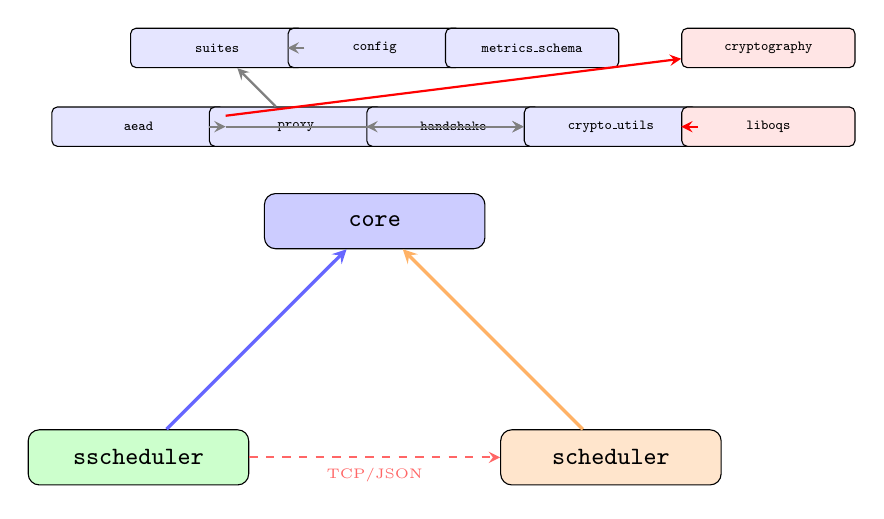
\begin{tikzpicture}[
    pkg/.style={draw, fill=#1, rounded corners, minimum width=2.8cm,
                minimum height=0.7cm, font=\small},
    mod/.style={draw, fill=#1, rounded corners=2pt, minimum width=2.2cm,
                minimum height=0.5cm, font=\tiny},
    dep/.style={->, thick, >=stealth, gray},
    node distance=0.7cm,
  ]
    % Packages
    \node[pkg=blue!20] (core)  at (0, 0)    {\texttt{core}};
    \node[pkg=green!20] (ssch) at (-3, -3)  {\texttt{sscheduler}};
    \node[pkg=orange!20] (sch) at (3, -3)   {\texttt{scheduler}};
    
    % Core modules
    \node[mod=blue!10] (aead)   at (-3, 1.2) {\texttt{aead}};
    \node[mod=blue!10] (proxy)  at (-1, 1.2) {\texttt{proxy}};
    \node[mod=blue!10] (hs)     at (1, 1.2)  {\texttt{handshake}};
    \node[mod=blue!10] (crypto) at (3, 1.2)  {\texttt{crypto\_utils}};
    \node[mod=blue!10] (suites) at (-2, 2.2) {\texttt{suites}};
    \node[mod=blue!10] (config) at (0, 2.2)  {\texttt{config}};
    \node[mod=blue!10] (schema) at (2, 2.2)  {\texttt{metrics\_schema}};
    
    % Internal core deps
    \draw[dep] (proxy)  -- (aead);
    \draw[dep] (proxy)  -- (hs);
    \draw[dep] (proxy)  -- (crypto);
    \draw[dep] (proxy)  -- (suites);
    \draw[dep] (aead)   -- (crypto);
    \draw[dep] (suites) -- (config);
    
    % Cross-package deps
    \draw[dep, blue!60, very thick] (ssch) -- (core);
    \draw[dep, orange!60, very thick] (sch) -- (core);
    \draw[dep, red!60, dashed] (ssch) -- node[below, font=\tiny] {TCP/JSON} (sch);
    
    % External
    \node[mod=red!10] (oqs) at (5, 1.2) {\texttt{liboqs}};
    \node[mod=red!10] (cry) at (5, 2.2) {\texttt{cryptography}};
    \draw[dep, red] (crypto) -- (oqs);
    \draw[dep, red] (aead) -- (cry);
  \end{tikzpicture}
  \caption{Cross-package dependency graph.  Solid arrows = Python import.
           Dashed red = network (TCP/JSON) dependency.}
  \label{fig:api-dependency-graph}
\end{figure}

% ====================================================================
\section{Summary Statistics}
\label{sec:api-summary}

\begin{table}[H]
  \centering
  \caption{Codebase summary statistics.}
  \label{tab:api-summary-stats}
  \begin{tabular}{l r}
    \toprule
    \textbf{Metric} & \textbf{Value} \\
    \midrule
    Total Python modules        & 37 \\
    Total lines of code         & $\sim$17{,}000 \\
    Public classes               & $\sim$60 \\
    Public methods/functions     & $\sim$250 \\
    Dataclass definitions        & $\sim$35 \\
    Enum types                   & 3 \\
    Exception classes            & 12 \\
    Configuration keys           & $\sim$100 \\
    Metric categories            & 18 (A--R) \\
    Supported cipher suites      & 216 \\
    External C library deps      & 1 (liboqs) \\
    External Python deps         & 4 (cryptography, psutil, ascon, pymavlink) \\
    \bottomrule
  \end{tabular}
\end{table}
